%!TEX root = mieic.tex
\chapter{Metodologia} \label{chap:metod}

\section*{}

Neste capítulo é descrita de uma forma sucinta a metodologia que será usada para alcançar os objetivos finais, que será baseada na interação pessoa-ecrã público. É incluída uma pequena descrição, definições e terminologias e ainda as diferentes fases para atingir o desejado. 

\section{Definições e Terminologia}

Considerando o cerne da questão, será adequado considerar dois coneitos relacionados, sendo eles Interação Pessoa-Computador e Desenvolvimento Centrado no Utilizador.

IHP tenta perceber como os utilizadores interagem com um computador, foca-se em perceber qual a melhor forma de projetar os sistemas interativos de forma mais agradável para quem usufrui dos mesmos.

Existem algumas rasões que fazem com que IHP seja uma área de estudo com valor~\cite{smith2006human}:
\begin{itemize}
	\item Considera como principal no desenvolvimento de aplicações o utilizador final e preocupa-se com ele aquando da fase de desenvolvimento.
	\item Fornece uma base sobre a qual é possível avaliar métodos de design para a sua eficiência e eficácia. O desenvolvimento de um sistema necessita de várias formas de avaliar os métodos usados, que podem ser obtidos através de IHP.
	\item Proporciona um ambiente baseado no mundo real, permitindo novas teorias baseadas na psicologia humana. este campo é uma das áreas de crescimento mais rápido considerando a ciência da computação.
\end{itemize}

DCU é um conceito para descrever os projectos nos quais o utilizador final influencia a forma como um projeto se desenvolve. É ao mesmo tempo uma filosofia ampla com vários métodos, pois há diversas maneiras através das quais os utilizadores são envolvidos. Uma metodologia baseada em UCD interessa-se pelas necessidades dos mesmos e frequentemente envolve-os durante o processo de design, normalmente durante o levantamento de requisitos e testes de usabilidade~\cite{Abras2004}.


\section{Fases de Desenvolvimento}

Uma vez que a metodologia é baseada no utilizador final é importante desenvolver um sistema intuitivo e de fácil utilização aos seus utilizadores.Um desnvolvimento centrado no utilizador final pressupõe 4 fases(figura ~\ref{fig:user-center}), sendo elas:
\begin{itemize}
\item Analisar - Engloba a recolha de requisitos, tendo em conta o contexto de uso e o propósito de desenvolvimento
\item Design - Projeta possíveis soluções que cumpram o que foi definido na fase anterior;
\item Implementar - Desenvolvimento de protótipos que tornem perceptiveis as soluções idealizadas, nos quais os conceitos têm de ser implementados.
\item Validar - Avaliação, por parte de especialistas, da usabilidade e possíveis riscos tendo em conta os requisitos do utilizador final e os conceitos envolvidos.
\end{itemize} 

\begin{figure}[h]
\centering
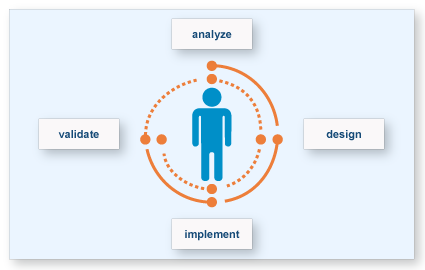
\includegraphics[width=0.7\columnwidth]{user.png}
\caption[Desenvolvimento Centrado no Utilizador] {Desenvolvimento Centrado no Utilizador\protect\footnotemark}
\label{fig:user-center}
\end{figure}

\footnotetext{http://www.medical-safety-design.de/en/medical-safety-design/user-centered-interface-design/}




